% figure to illustrate match a substring in a text.
\ifdefined\includetikz\relax \else
%\documentclass{standalone}
\documentclass{article}
\usepackage{tikz}
\usepackage{amsmath}
\usetikzlibrary{matrix,backgrounds,positioning}
\begin{document}
\fi

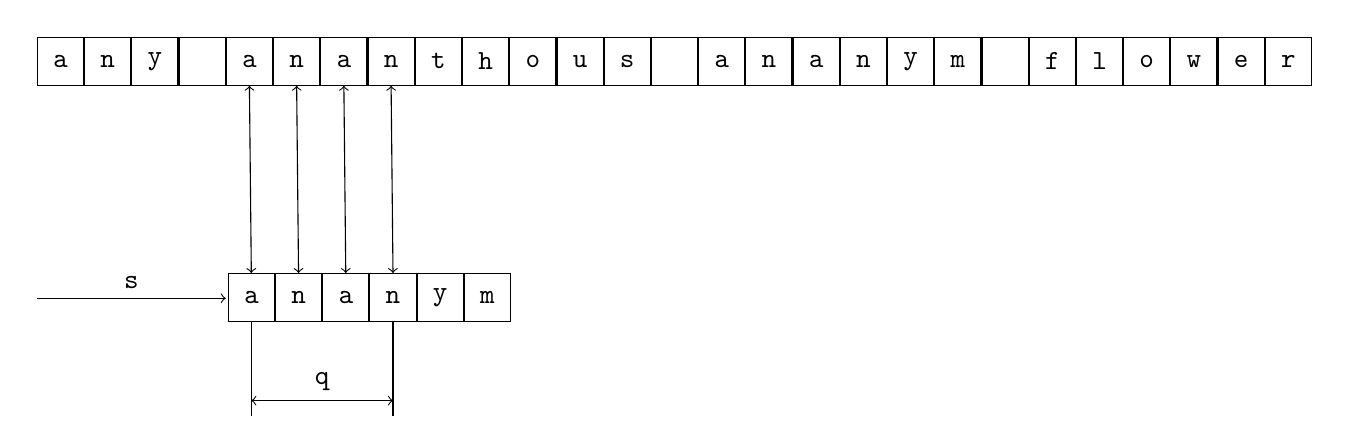
\begin{tikzpicture}[font=\ttfamily,
scale=1,
array/.style={matrix of nodes,
              nodes={draw, align=center, anchor=south, minimum height = 4ex, text width=1em},
              %column sep=-\pgflinewidth,
              %row sep=0.5mm,
              nodes in empty cells
              %row 1/.style={nodes={draw=none, fill=none, minimum size=5mm}},
              %row 1 column 1/.style={nodes={draw}}
              }]

%any ananthous ananym flower
\matrix[array] (array) {
a & n & y & & a & n & a & n & t & h & o & u & s & & a & n & a & n & y & m & & f & l & o & w & e & r \\};

%ananym
\matrix[array,
  anchor=west] at ([yshift=-3cm, xshift=-0.4cm]array-1-5) (myptn) {
a & n & a & n & y & m \\};

% offset s
\draw[->] ([yshift=-2.7cm]array-1-1.south west) -- node[above] {s} ([yshift=-2.7cm]array-1-4.south east);

% matches chars so far.
\foreach \i/\j in {5/1, 6/2, 7/3, 8/4} {
  \draw[<->] (array-1-\i.south) -- (myptn-1-\j.north);
}

% matched count q.
\draw (myptn-1-1.south) -- ++(0, -1.2cm);
\draw (myptn-1-4.south) -- ++(0, -1.2cm);
\draw[<->] ([yshift=-1cm]myptn-1-1.south) -- node[above] {q} ([yshift=-1cm]myptn-1-4.south);

\end{tikzpicture}

\ifdefined\includetikz\relax \else
\end{document}
\fi
